\documentclass[11pt]{scrartcl}

\usepackage[top=1.5cm]{geometry}
\usepackage{url}
\usepackage{float}
\usepackage{listings}
\usepackage{xcolor}
\usepackage{graphicx}
\usepackage{amsmath}

\setlength{\parindent}{0em}
\setlength{\parskip}{0.5em}

\newcommand{\youranswerhere}{[Your answer goes here \ldots]}
\renewcommand{\thesubsection}{\arabic{subsection}}

\lstdefinestyle{dmrsql}{
  language=SQL,
  basicstyle=\small\ttfamily,
  keywordstyle=\color{magenta!75!black},
  stringstyle=\color{green!50!black},
  showspaces=false,
  showstringspaces=false,
  commentstyle=\color{gray}}

\lstdefinestyle{dmrPython}{
  language=PYTHON,
  basicstyle=\small\ttfamily,
  keywordstyle=\color{magenta!75!black},
  stringstyle=\color{green!50!black},
  showspaces=false,
  showstringspaces=false,
  commentstyle=\color{gray}}

\title{
  \textbf{\large Projektaufgabe 2 } \\
  Phase 1 – Legen der Basis (2.5 P) \\
  {\large Datenmanagement jenseits von Relationen}
}

\author{
  Gruppen Nummer (A17) \\
  \large Acikyol Aleyna, 12032843 \\
  \large Özcan Ahmet, 12311287 \\
  \large Sadykova Nargiz, 12129337 \\
}

\begin{document}

\maketitle\thispagestyle{empty}

Dieses Reporting Template dient der Vorbereitung der Abgabe von Phase 1.

\subsection*{Datengenerator für Matrizen mit Sparsity (0.5 Punkte)}

Zeigen Sie den Code der Funktion generate() als Listing oder Screenshot. Gehen Sie
(kurz) auf die wesentlichen Aspekte ein

{Die Funktion generate(l, sparsity) erzeugt zwei nahezu quadratische Matrizen A und B als 2D-Arrays mit Gleitkommazahlen. Aus dem Größenparameter l werden die Dimensionen m = l - 1 und n = l - 1 berechnet, sodass A die Größe (l-1) × l und B die Größe l × (l-1) besitzt. Die Matrixeinträge werden zunächst mit zufälligen double-Werten erzeugt; in Python entsprechen die verwendeten float-Werte der double-Genauigkeit. Anschließend wird für jede Matrix aus der Gesamtanzahl der Zellen und dem Parameter sparsity die Anzahl der Nullwerte bestimmt. Diese Nullwerte werden zufällig auf die möglichen Matrixpositionen verteilt, indem alle Indexpunkte (i, j) erzeugt, gemischt und die berechnete Anzahl davon auf 0.0 gesetzt wird. Die Funktion gibt beide Matrizen als Rückgabewert zurück.}

\begin{lstlisting}[style=dmrPython]
import random

def generate(l, sparsity):
    if l < 2:
        raise ValueError("l muss mindestens 2 sein")
    if not (0.0 <= sparsity <= 1.0):
        raise ValueError("sparsity muss zwischen 0 und 1 liegen")

    m = l - 1
    n = l - 1

    # A: m x l
    A = [[random.uniform(1.0, 10.0) for _ in range(l)] for _ in range(m)]
    # B: l x n
    B = [[random.uniform(1.0, 10.0) for _ in range(n)] for _ in range(l)]

    total_A = m * l
    total_B = l * n

    zeros_in_A = round(sparsity * total_A)
    zeros_in_B = round(sparsity * total_B)

    positions_A = [(i, j) for i in range(m) for j in range(l)]
    positions_B = [(i, j) for i in range(l) for j in range(n)]

    random.shuffle(positions_A)
    random.shuffle(positions_B)

    for i, j in positions_A[:zeros_in_A]:
        A[i][j] = 0.0
    for i, j in positions_B[:zeros_in_B]:
        B[i][j] = 0.0

    return A, B
\end{lstlisting}

\subsection*{Import der Matrizen in das DBMS (0.5 Punkte):}

Geben Sie das Create Table Statement für Matrix A an.

\begin{lstlisting}[style=dmrsql]
CREATE TABLE A (
    i INT,
    j INT,
    val DOUBLE PRECISION
);
import psycopg2
from psycopg2.extras import execute_values

def import_to_db(matrix, table_name, db_config):
    # Daten vorbereiten
    sparse_data = []
    for i in range(len(matrix)):
        for j in range(len(matrix[0])):
            if matrix[i][j] != 0.0:
                sparse_data.append((i + 1, j + 1, matrix[i][j]))

    # Verbindung und Import
    conn = psycopg2.connect(**db_config)
    cursor = conn.cursor()

    query = f"INSERT INTO {table_name} (i, j, val) VALUES %s"
    execute_values(cursor, query, sparse_data)

    conn.commit()
    cursor.close()
    conn.close()
    print(f"Import in {table_name} erfolgreich!")
\end{lstlisting}

Für die Übung bereiten Sie eine Demo des Datenimports vor.


\subsection*{Wahl des Toy Beispiels (0.5 P):}

Geben Sie Matrix A und B als 2D Array an.

Matrix A: \\
\begin{bmatrix}
  1  &  0  &  3 \\
  0  &  7  &  8 \\
  9  &  8  &  0 \\
  4  &  0  &  2
\end{bmatrix}
\\\\
Matrix B:\\
\begin{bmatrix}
  5  &  0  &  7  &  10  &  4 \\
  8  &  9  &  1  &  0  &  8 \\
  4  &  0  &  0  &  2  &  1
\end{bmatrix}

Zeigen Sie die äquivalente Darstellung der Matrix A und B in der Datenbank

\begin{figure}[H]
    \centering
    \begin{minipage}{0.45\textwidth}
        \centering
        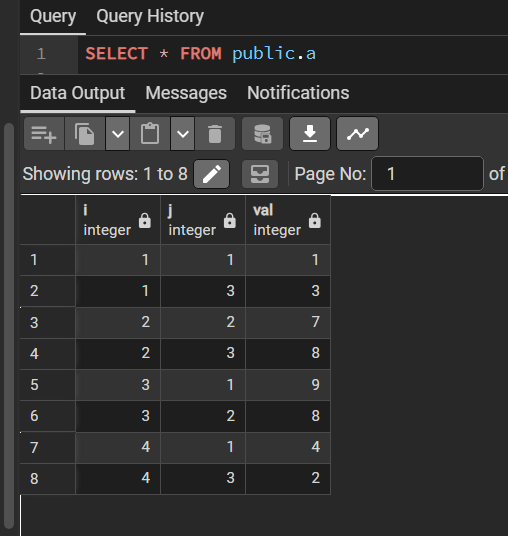
\includegraphics[width=\textwidth]{2-3_MatrixA.png}
        \caption{Matrix A}
    \end{minipage}
    \hfill
    \begin{minipage}{0.45\textwidth}
        \centering
        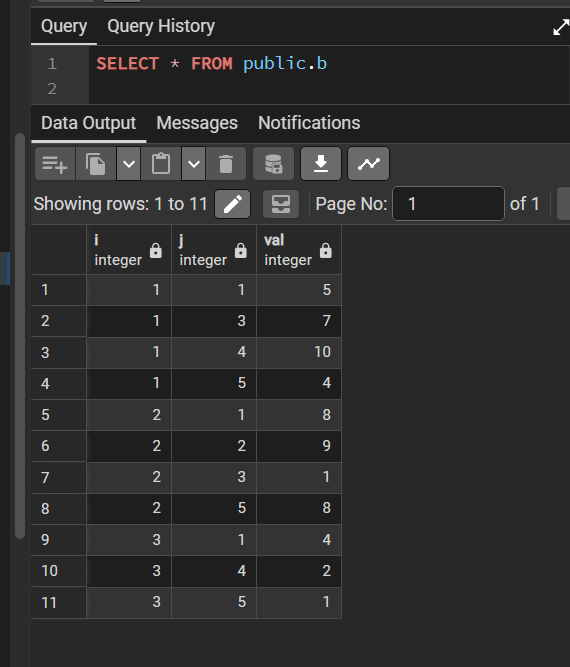
\includegraphics[width=\textwidth]{2-3_MatrixB.png}
        \caption{Matrix B}
    \end{minipage}
\end{figure}

\subsection*{Implementierung von Ansatz 0 (0.5 P):}
Zeigen Sie den Code der Matrixmultiplikation als Listing oder Screenshot. Erläutern Sie (kurz), welche Laufzeit ihr Algorithmus hat und warum das Kriterium keinen Algorithmus mit sub-kubischer Laufzeit zu wählen erfüllt ist

\begin{lstlisting}[style=dmrPython]
# A 4x3 (mxl)
a = [
    [1, 0, 3],
    [0, 7, 8],
    [9, 8, 0],
    [4, 0, 2]
]

# B 3x5 (lxn)
b = [
    [5, 0, 7, 10, 4],
    [8, 9, 1, 0, 8],
    [4, 0, 0, 2, 1]
]


def matrixmult(A, B):
    """C = A x B auf Client-Seite (also reine Mathe)"""

    m = len(A)
    l = len(A[0])
    n = len(B[0])

    #befuelle C (mxn) mit Nullern
    C = [[0] * n for _ in range(m)]

    for i in range(m):
        for k in range(l):
            for j in range(n):
                C[i][j] += A[i][k] * B[k][j]

    return C

# Test mit Toy-Beispiel
c_result = matrixmult(a, b)

print("\nErgebnis C = A x B (Ansatz 0):")
for row in c_result:
    print(row)
\end{lstlisting}
Die Laufzeit des Algorithmus von $matrixmult$ beträgt O($n^3$). Dies wird durch die dreifache $for$-Schleife ermöglicht. \\
Die Schleifen durchlaufen die Reihen von A (auch als $m$ bezeichnet, hier $4$ Reihen), die Spalten von A (welche gleich lang zu den Reihen von B ist; hier markiert als $l$) und die Spalten von B (gekennzeichnet als $n$).

\subsection*{Implementierung von Ansatz 1 (0.5 P):}

Ansatz 1 berechnet $C = A \times B$ direkt im DBMS auf Basis der Sparse-Darstellung
der Tabellen \texttt{A(i, j, val)} und \texttt{B(i, j, val)}.
Der Join über \texttt{A.j = B.i} entspricht dem inneren Produkt der Matrixmultiplikation.
Das Ergebnis wird nicht persistent gespeichert.

\begin{lstlisting}[style=dmrsql]
SELECT A.i, B.j, SUM(A.val * B.val)
FROM A, B
WHERE A.j = B.i
GROUP BY A.i, B.j
ORDER BY A.i, B.j;
\end{lstlisting}

Das handberechnete Ergebnis $C = A \times B$ für das Toy-Beispiel lautet:

\[
C = \begin{pmatrix}
 17 &  0 &  7 & 16 &   7 \\
 88 & 63 &  7 & 16 &  64 \\
109 & 72 & 71 & 90 & 100 \\
 28 &  0 & 28 & 44 &  18
\end{pmatrix}
\]

Zeigen Sie, dass Ihr System $C$ korrekt berechnet (z.B. als Screenshot)

Die Korrektheitsprüfung erfolgt durch Ausführen von \texttt{Task2-6-Korrektheitspruefung.py},
welches Ansatz~0 und Ansatz~1 auf dem Toy-Beispiel ausführt und die Ergebnisse vergleicht.
Beide Ansätze liefern das identische Ergebnis:

\begin{lstlisting}[style=dmrsql]
Ansatz 0 == erwartet: True
Ansatz 1 == erwartet: True
Ansatz 0 == Ansatz 1: True
\end{lstlisting}

\subsection*{Zeitmamagement}

Benötigte Zeit pro Person (nur Phase 1): \textbf{Aleyna Acikyol: 4.5 Stunden, Ahmet Özcan: 4 Stunden, Nargiz Sadykova: 3.5 Stunden.}

\end{document}
